\documentclass[]{article}
\usepackage{graphicx}
\usepackage[usenames,dvipsnames]{xcolor}
\usepackage{braket}
\usepackage{array}
\usepackage{tikz}
\usepackage[a4paper,twoside,left=35mm,right=25mm,top=40mm,bottom=35mm]{geometry}
\usepackage{pgfplots}
\begin{document}
\begin{figure}
(a) \hspace{2.5cm} (i)  $t = 1000 ~(\xi/c)$ \hspace{2.4cm} \hspace{1.8cm} (ii)   $t= 3500~ (\xi/c)$
\\
\begin{tikzpicture}
  \begin{axis}[
      axis on top,
      width=0.5\linewidth,
      xlabel=$x/\xi$,
      ylabel=$y/\xi$,
      unit vector ratio=1 1 1,
      xmin = 150,
      xmax = 380,
      ymin = -45,
      ymax = 45,
      major tick length = 0.07cm,
    ]
    \addplot graphics [xmin=150,xmax=380,ymin=-45,ymax=45] {wake/figure2ai-dens};
  \end{axis}
\end{tikzpicture}
\begin{tikzpicture}
  \begin{axis}[
      axis on top,
      width=0.5\linewidth,
      xlabel=$x/\xi$,
      ylabel=$y/\xi$,
      unit vector ratio=1 1 1,
      xmin = 150,
      xmax = 380,
      ymin = -45,
      ymax = 45,
      major tick length = 0.07cm,
    ]
    \addplot graphics [xmin=150,xmax=380,ymin=-45,ymax=45] {wake/figure2aii-dens};
  \end{axis}
\end{tikzpicture}

\vspace{0.2cm}
(b)\hspace{2.5cm} (i)  $t = 0-1500 ~(\xi/c)$ \hspace{2.4cm} \hspace{1.2cm} (ii)   $t= 3500~ (\xi/c)$
\\
\vspace{0.3cm}
\begin{tikzpicture}
  \begin{axis}[
      axis on top,
      width=0.5\linewidth,
      xlabel=$x/\xi$,
      ylabel=$y/\xi$,
      unit vector ratio=1 1 1,
      xmin = 150,
      xmax = 380,
      ymin = -45,
      ymax = 45,
      major tick length = 0.07cm,
    ]
    \addplot graphics [xmin=150,xmax=380,ymin=-45,ymax=45] {wake/figure2bi-raw};
  \end{axis}
\end{tikzpicture}
  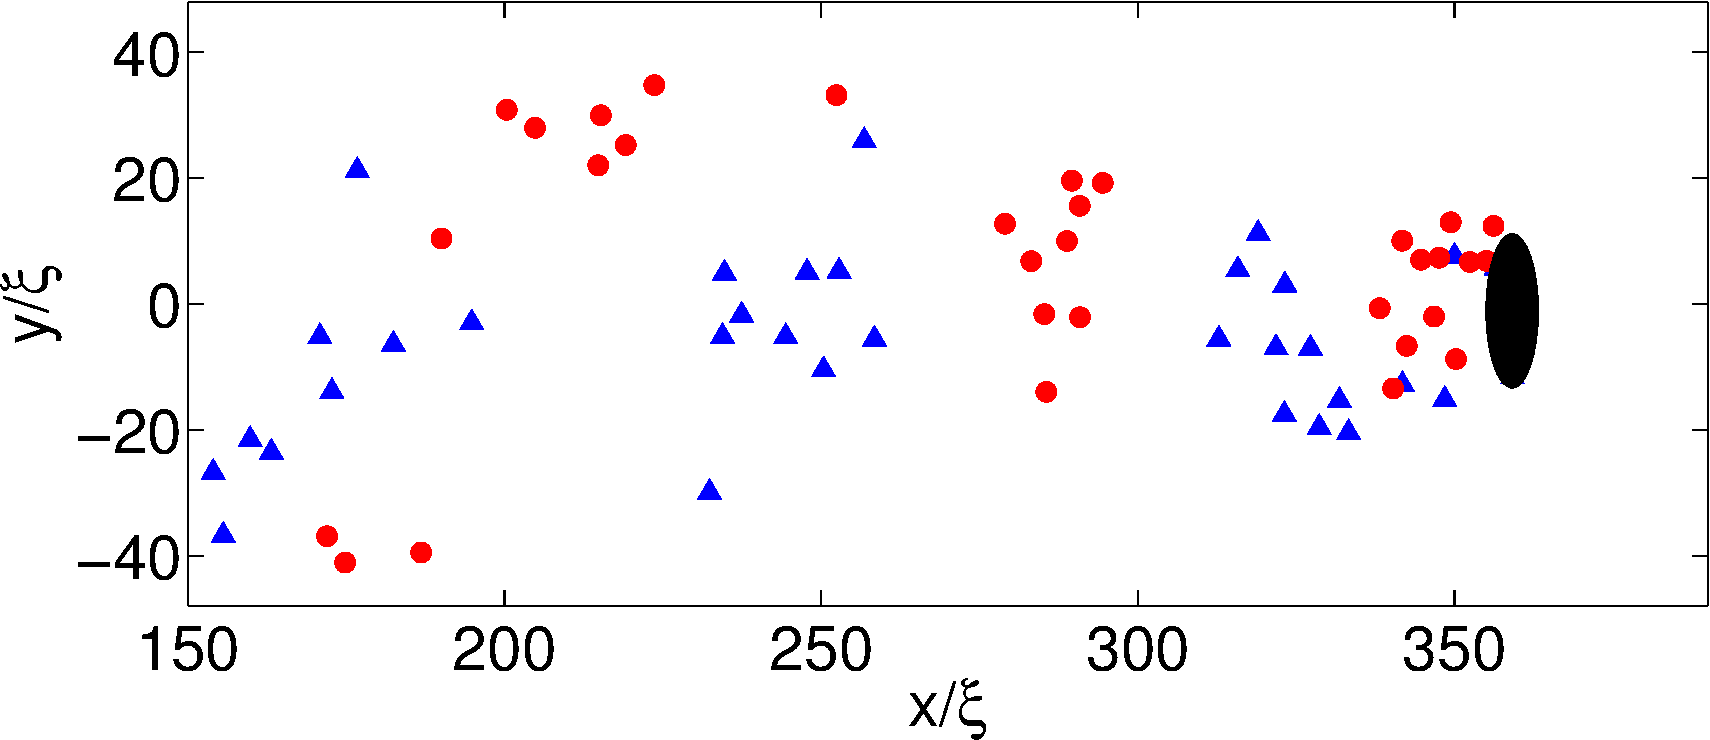
\includegraphics[width=0.5\textwidth]{wake/figure2bii}
  \caption{Snapshots showing the (a) density profile and (b) vortex trajectories during vortex shedding from an elliptical object ($\varepsilon = 3$) at (i) early times and (ii) later times.  The obstacle has speed $v=0.52c$ and size $d = 5\xi$. Red and blue lines represent vortices of oppositely quantized circulation. At early $t$, a symmetric wake similar to a classical fluid with low $Re$ forms. Symmetry breaks at $t\approx1500~(\xi/c)$ at which point vortex motion becomes disordered. In this case the initial condition is noise-free.}
  \label{fig:denstraj}
\end{figure}



\end{document}
